\documentclass{article}
\usepackage{amsmath}
\usepackage{amssymb}
\usepackage{graphicx}
\usepackage{hyperref}
\usepackage[version=4]{mhchem}


\begin{document}
\(A B C D\) is a rectangle with \(A B=2 B C\). \(E\) and \(F\) are the midpoints of \(A B\) and \(A D\), respectively. \(D E\) and \(B F\) meet at \(G\). What is the ratio of the area of \(G B C D\) to the area of \(A B C D\) ?\\
(A) \(\frac{5}{2}\)\\
(B) \(\frac{2}{5}\)\\
(C) \(\frac{2}{3}\)\\
(D) \(\frac{4}{5}\)\\
(E) \(\frac{3}{5}\)\\
\centering
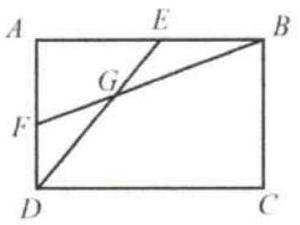
\includegraphics[width=\textwidth]{images/011.jpg}

Solution: (C).\\
We connect \(B D\) and extend \(A G\) to meet \(B D\) at \(H\).\\
Since the medians \(D E\) and \(B F\) meet at \(G, G\) is the centroid of triangle \(A B D\) and the six small triangles formed have the same area.\\
\centering
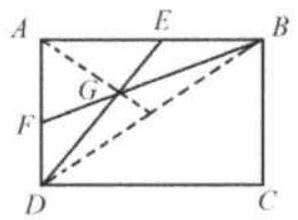
\includegraphics[width=\textwidth]{images/011(1).jpg}

Each of the small triangles has an area that is \(\frac{1}{12}\) of the area of the rectangle \(A B C D\), so the area of triangle \(D B G, S_{D G B}=\frac{2}{12} \times S_{A B C D}\).\\
The area of triangle \(D B C, S_{D B C}=\frac{1}{2} \times S_{A B C D}\).\\
\(S_{D C B C}=S_{D C B}+S_{D B C}=\frac{2}{12} S_{A B C D}+\frac{1}{2} S_{A B C D}=\left(\frac{2}{12}+\frac{1}{2}\right) \times S_{A B C D}\).\\
The ration of the area of \(G B C D\) to the area of \(A B C D\).\\
\(S_{D C B C}=\frac{S_{D C B C}}{S_{A B C D}}=\frac{2}{12}+\frac{1}{2}=\frac{2+6}{12}=\frac{2}{3}\).


\end{document}
